% vim: foldmethod=marker: 
\documentclass[11pt]{standalone}

\usepackage[utf8]{inputenc}
\usepackage[T1]{fontenc}    


\usepackage{tikz}
\usetikzlibrary{snakes} %% produces curly arrows on tikz
\usetikzlibrary{matrix} %% for commutative diagrams
\usetikzlibrary{arrows}

\usepackage{ifthen}

\begin{document}
    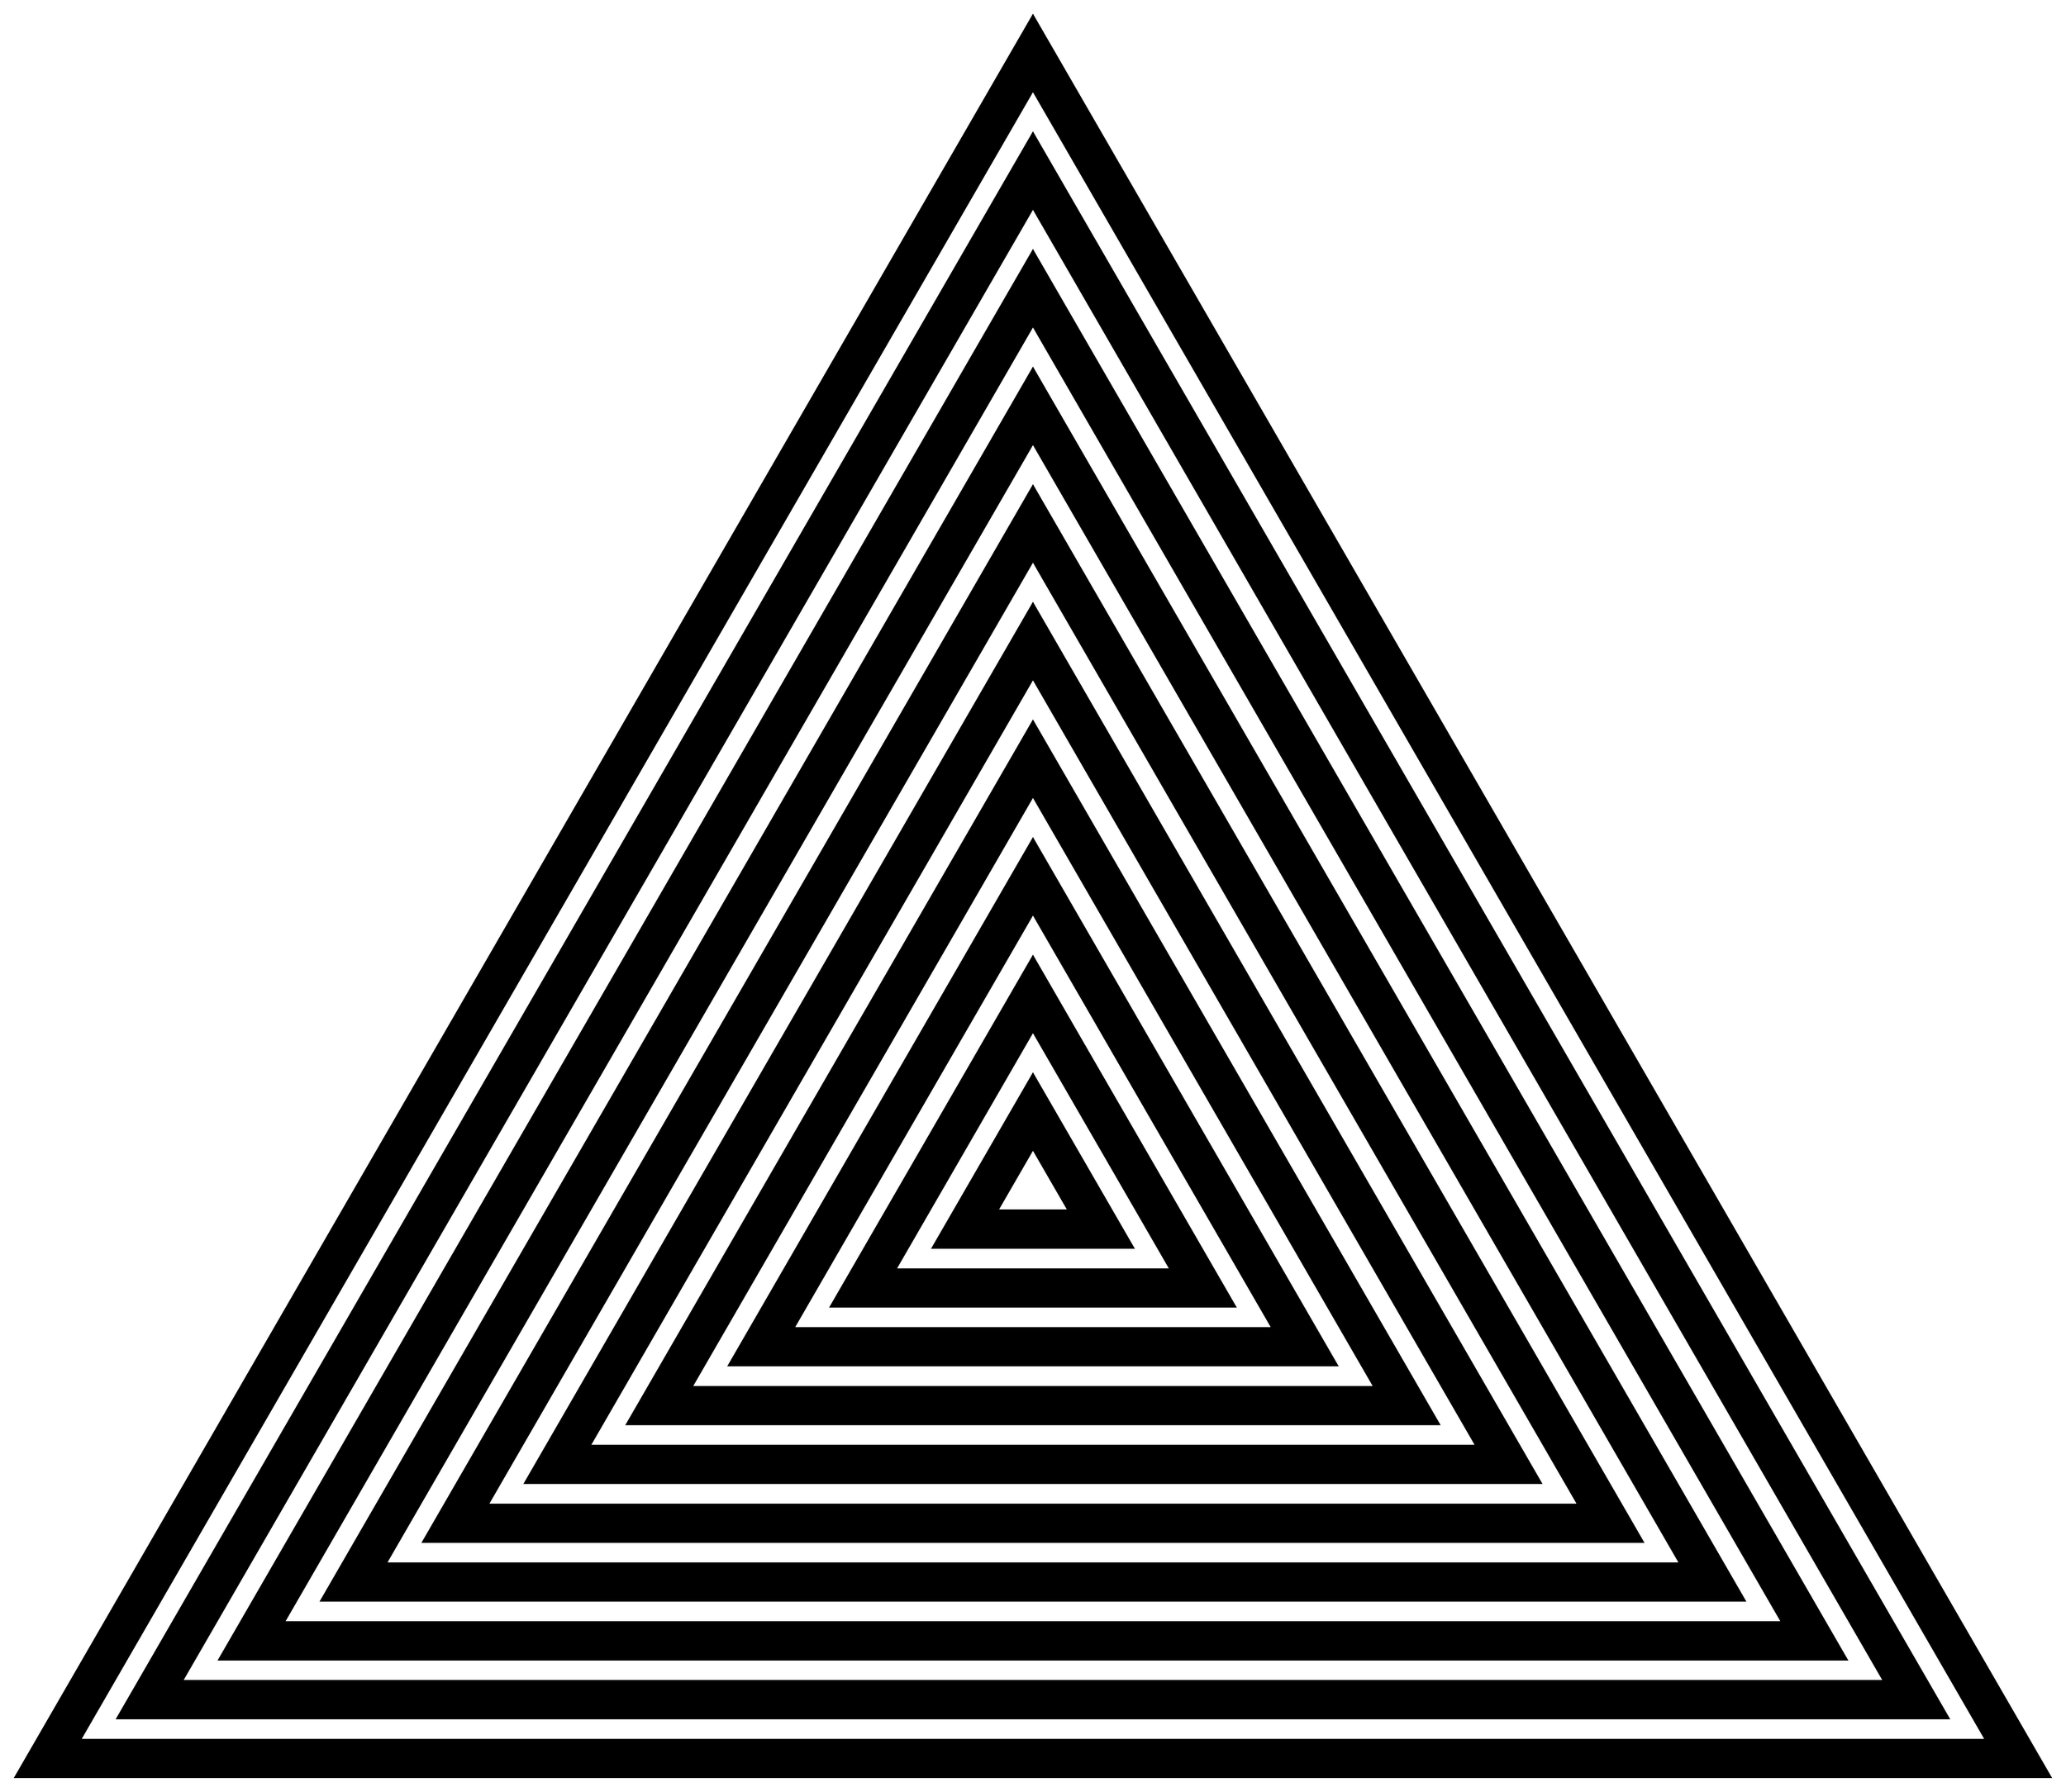
\begin{tikzpicture}
        \foreach \ra in {30,27,..., 3} {
            \pgfmathsetmacro\rb{\ra-2}
            \fill[black, even odd rule ]
                (90:\ra) -- (210:\ra) -- (-30:\ra) -- cycle
                (90:\rb) -- (210:\rb) -- (-30:\rb) -- cycle;
        }
    \end{tikzpicture}
\end{document}


